\documentclass[11pt,a4paper]{article}

\usepackage[utf8]{inputenc}
\usepackage[margin=1in]{geometry}
\usepackage{amsmath,amssymb}
\usepackage{booktabs}
\usepackage{graphicx}
\usepackage{hyperref}
\usepackage{cite}
\usepackage{listings}
\usepackage{xcolor}

\hypersetup{
    colorlinks=true,
    linkcolor=blue,
    citecolor=blue,
    urlcolor=blue
}

\lstset{
    basicstyle=\ttfamily\footnotesize,
    keywordstyle=\color{blue}\bfseries,
    stringstyle=\color{teal},
    commentstyle=\color{gray}\itshape,
    breaklines=true,
    frame=single,
    captionpos=b
}

\title{\textbf{AutoGrammar: Machine Learning-Based Automatic Grammar Inference for Domain-Specific Languages with MySQL Integration}}

\author{
    \textbf{AutoGrammar Research \& Development Team} \\
    Department of Computer Science \& Compiler Engineering \\
    Academic Project Report
}

\date{\today}

\begin{document}

\maketitle

\begin{abstract}
Domain-Specific Languages (DSLs) provide tailored, expressive formalisms for specialized software domains such as database querying and student information management. However, authoring and maintaining formal context-free grammars for evolving DSLs is traditionally labor-intensive and prone to human error. In this paper, we present \textbf{AutoGrammar}, an end-to-end framework integrating machine learning-based grammar induction with compiler design and relational database execution. Using a culturally authentic synthetic dataset of 10,000 Indian school student records and 7,000 SQL-like DSL queries, AutoGrammar automatically infers Extended Backus-Naur Form (EBNF) grammar productions from tokenized exemplars. We prevent data leakage through template-level disjoint partitioning across training (70\%), validation (15\%), and held-out test (15\%) splits. In experimental evaluations on 1,146 held-out test queries, the automatically inferred grammar achieves an overall parsing accuracy of 89.53\% (85.71\% valid query acceptance and 100.0\% invalid query rejection) with an EBNF production F1-score of 0.9873 relative to a manually authored reference grammar. In contrast, an n-gram TF-IDF statistical baseline achieves only 66.67\% accuracy with a high False Acceptance Rate (84.0\%) on invalid queries. AutoGrammar incorporates schema-aware semantic validation and execution guardrails connected to MySQL 8.0 and a relational sandbox.
\end{abstract}

\section{Introduction}
Domain-Specific Languages (DSLs) simplify domain operations by constraining syntax to purposeful semantics. In educational administration, SQL subsets frequently serve as declarative DSLs for querying student records, marks, and attendance. Building robust parsers for such DSLs typically requires compiler engineers to manually specify grammar productions using tools such as Lex/Yacc, ANTLR, or Lark \cite{aho2006compilers}. When language requirements evolve, updating these specifications manually creates synchronization overhead and syntactic ambiguity.

Grammar induction (also known as grammatical inference) addresses this challenge by algorithmically learning formal syntax rules directly from corpora of sample sentences \cite{degroote2010grammatical}. However, conventional grammatical inference algorithms often operate as abstract formalisms without integration into executable compiler pipelines or real-world database systems. Furthermore, purely statistical machine learning models (such as bag-of-words or TF-IDF classifiers) cannot output structural parse trees and frequently accept malformed sequences that lack grammatical ordering.

To bridge this gap, this project develops \textbf{AutoGrammar}, a fully implemented, runnable compiler and grammar-induction system. The key contributions of this work include:
\begin{enumerate}
    \item \textbf{Synthetic Indian School Dataset}: A reproducible relational database generator producing 10,000 student records and 7,000 SQL DSL queries categorized into valid and systematically invalid patterns across 16 grammatical categories.
    \item \textbf{Leakage-Free Partitioning}: A template-based grouping strategy guaranteeing that identical structural templates never appear in both training and evaluation splits.
    \item \textbf{Automatic Grammar Induction Engine}: A rule induction algorithm that abstracts tokens, detects recurring skeletons, establishes precedence, and synthesizes valid Lark EBNF grammars.
    \item \textbf{4-Stage Compiler Pipeline}: Deterministic lexical analysis, syntax parsing, schema-aware semantic checking, and execution safety guardrails.
    \item \textbf{Empirical Comparison}: Comparative evaluation between the reference baseline grammar, the automatically induced grammar, and an ML statistical classifier.
\end{enumerate}

\section{Related Work}
Grammatical inference has a rich theoretical foundation dating back to Gold's identification in the limit and Angluin's $L^*$ algorithm for regular languages \cite{angluin1987learning, degroote2010grammatical}. While classic automata learning concentrates on regular languages (DFAs), natural languages and database query structures exhibit context-free nested characteristics necessitating Context-Free Grammars (CFGs).

Recent research in semantic parsing and natural language interfaces to databases (NLIDB) has popularized deep learning models such as Seq2SQL \cite{zhong2017seq2sql} and Spider benchmarks \cite{yu2018spider}. Although neural models excel at translation, they frequently suffer from hallucinations, non-deterministic syntax violations, and opacity. In contrast, compiler engineering mandates deterministic guarantees, precise error localization (line and column numbers), and strict semantic validation \cite{aho2006compilers}. AutoGrammar combines the adaptive capability of induction with the rigor of deterministic compiler pipelines.

\section{Proposed Methodology}

\subsection{Relational Schema and Synthetic Corpus Generation}
The database schema (`school_db`) encompasses six normalized tables: `students`, `teachers`, `classes`, `subjects`, `marks`, and `attendance`. Culturally authentic fictional records are generated using regional Indian naming conventions spanning Andhra Pradesh, Telangana, Karnataka, Tamil Nadu, Kerala, Maharashtra, and Delhi.

\begin{table}[h]
\centering
\caption{AutoGrammar Dataset Scale and Structural Characteristics}
\label{tab:dataset_stats}
\begin{tabular}{llr}
\toprule
\textbf{Category} & \textbf{Entity / Split} & \textbf{Count} \\
\midrule
Relational Database & Synthetic Students & 10,000 \\
& Synthetic Teachers & 40 \\
& Synthetic Classes & 7 \\
& Synthetic Marks & 6,031 \\
& Synthetic Attendance & 6,000 \\
\midrule
Query Corpus & Total Synthesized Queries & 7,000 \\
& Valid Queries & 5,000 \\
& Invalid Queries & 2,000 \\
& Distinct Structural Templates & 68 \\
\midrule
Dataset Splits & Training Set (70\%) & 4,826 \\
& Validation Set (15\%) & 1,028 \\
& Held-Out Test Set (15\%) & 1,146 \\
\bottomrule
\end{tabular}
\end{table}

\subsection{Data Leakage Prevention}
A major vulnerability in machine learning evaluation is slot-filling data leakage, where queries sharing identical syntactic structures appear in both training and test sets with merely different literal constants. AutoGrammar prevents this by partitioning data strictly at the `template_id` level. Templates allocated to the training split are completely disjoint from those in validation and test sets.

\subsection{Grammar Induction Algorithm}
The induction algorithm operates in four sequential phases:
\begin{enumerate}
    \item \textbf{Tokenization and Canonicalization}: Queries are tokenized via `SqlLexer`. Keywords are preserved, while identifiers and literals are mapped to structural tokens.
    \item \textbf{Skeleton Discovery}: Clause sequences are mapped to topological patterns (e.g., $\text{SELECT} \rightarrow \text{FROM} \rightarrow \text{WHERE} \rightarrow \text{ORDER\_BY} \rightarrow \text{LIMIT}$).
    \item \textbf{EBNF Rule Synthesis}: Mandatory versus optional clauses are inferred. Suffix sequences such as `("," select_item)*` are generated for list structures. Operator precedence (`OR` over `AND` over `NOT`) is constructed hierarchically.
    \item \textbf{Validation and Compilation}: The candidate Lark specification is validated using Earley/LALR parser engines to guarantee zero syntax conflicts.
\end{enumerate}

\begin{lstlisting}[language=SQL, caption={Example Inferred Lark EBNF Grammar Production}]
select_stmt: "SELECT"i [distinct_clause] select_list from_clause [where_clause] [groupby_clause] [having_clause] [orderby_clause] [limit_clause]
distinct_clause: "DISTINCT"i
select_list: select_item ("," select_item)*
from_clause: "FROM"i table_source (join_clause)*
table_source: CNAME ["AS"i CNAME]
join_clause: (["INNER"i] "JOIN"i | "LEFT"i ["JOIN"i]) table_source "ON"i condition
where_clause: "WHERE"i condition
\end{lstlisting}

\subsection{Compiler Architecture and Safety Gate}
The compiler pipeline enforces four stages:
\begin{itemize}
    \item \textbf{Stage 0: Pre-Parse Security Gate}: Blocks forbidden administrative statements (`DROP`, `TRUNCATE`, `ALTER`) and multi-statement injection.
    \item \textbf{Stage 1: Lexical Analysis}: Validates tokens and tracks coordinate offsets.
    \item \textbf{Stage 2: Syntax Analysis}: Evaluates input against the active grammar and constructs parse trees.
    \item \textbf{Stage 3: Semantic Validation}: Resolves table and column references against the live schema and validates alias assignments.
\end{itemize}

\section{Results and Discussion}

\subsection{Experimental Performance Benchmarks}
We evaluated the systems on 1,146 held-out test queries derived from unseen templates.

\begin{table}[h]
\centering
\caption{Comparative Evaluation: Baseline Grammar vs. Learned Grammar vs. ML Classifier}
\label{tab:comparison}
\begin{tabular}{lrrrrr}
\toprule
\textbf{Paradigm} & \textbf{Accuracy} & \textbf{TPR (Recall)} & \textbf{TNR (Spec.)} & \textbf{FAR} & \textbf{FRR} \\
\midrule
Fixed Baseline Grammar & 100.00\% & 100.00\% & 100.00\% & 0.00\% & 0.00\% \\
\textbf{AutoGrammar Learned} & \textbf{89.53\%} & \textbf{85.71\%} & \textbf{100.00\%} & \textbf{0.00\%} & \textbf{14.29\%} \\
ML TF-IDF + Logistic Reg. & 66.67\% & 85.12\% & 16.01\% & 83.99\% & 14.88\% \\
\bottomrule
\end{tabular}
\end{table}

\subsection{Grammar Rule Induction Evaluation}
Comparing the learned grammar against the reference baseline grammar yields:
\begin{itemize}
    \item Reference Baseline Rules: 40
    \item Learned Rules: 39 (Shared matching rules: 39)
    \item Production Rule Precision: \textbf{1.0000}
    \item Production Rule Recall: \textbf{0.9750}
    \item Production Rule F1-Score: \textbf{0.9873}
\end{itemize}
The only rule absent from the initially learned grammar was `delete_stmt`, directly attributable to the strict template-level partitioning where `DELETE` exemplars were partitioned into the validation split. When tested through the interactive refinement loop, the system successfully induced `delete_stmt` upon presentation of an approved example.

\subsection{Analysis of ML Classifier Limitations}
As shown in Table \ref{tab:comparison}, the statistical TF-IDF classifier achieved an accuracy of only 66.67\% on the held-out test set, with 257 False Positives (False Acceptance Rate of 83.99\%). Because n-gram classification lacks structural grammar understanding, queries containing valid keywords in malformed sequences (e.g., missing `FROM` clauses or unbalanced parentheses) are misclassified as valid. AutoGrammar's formal parser completely eliminates false acceptances ($\text{FAR} = 0.00\%$).

\begin{figure}[h]
\centering
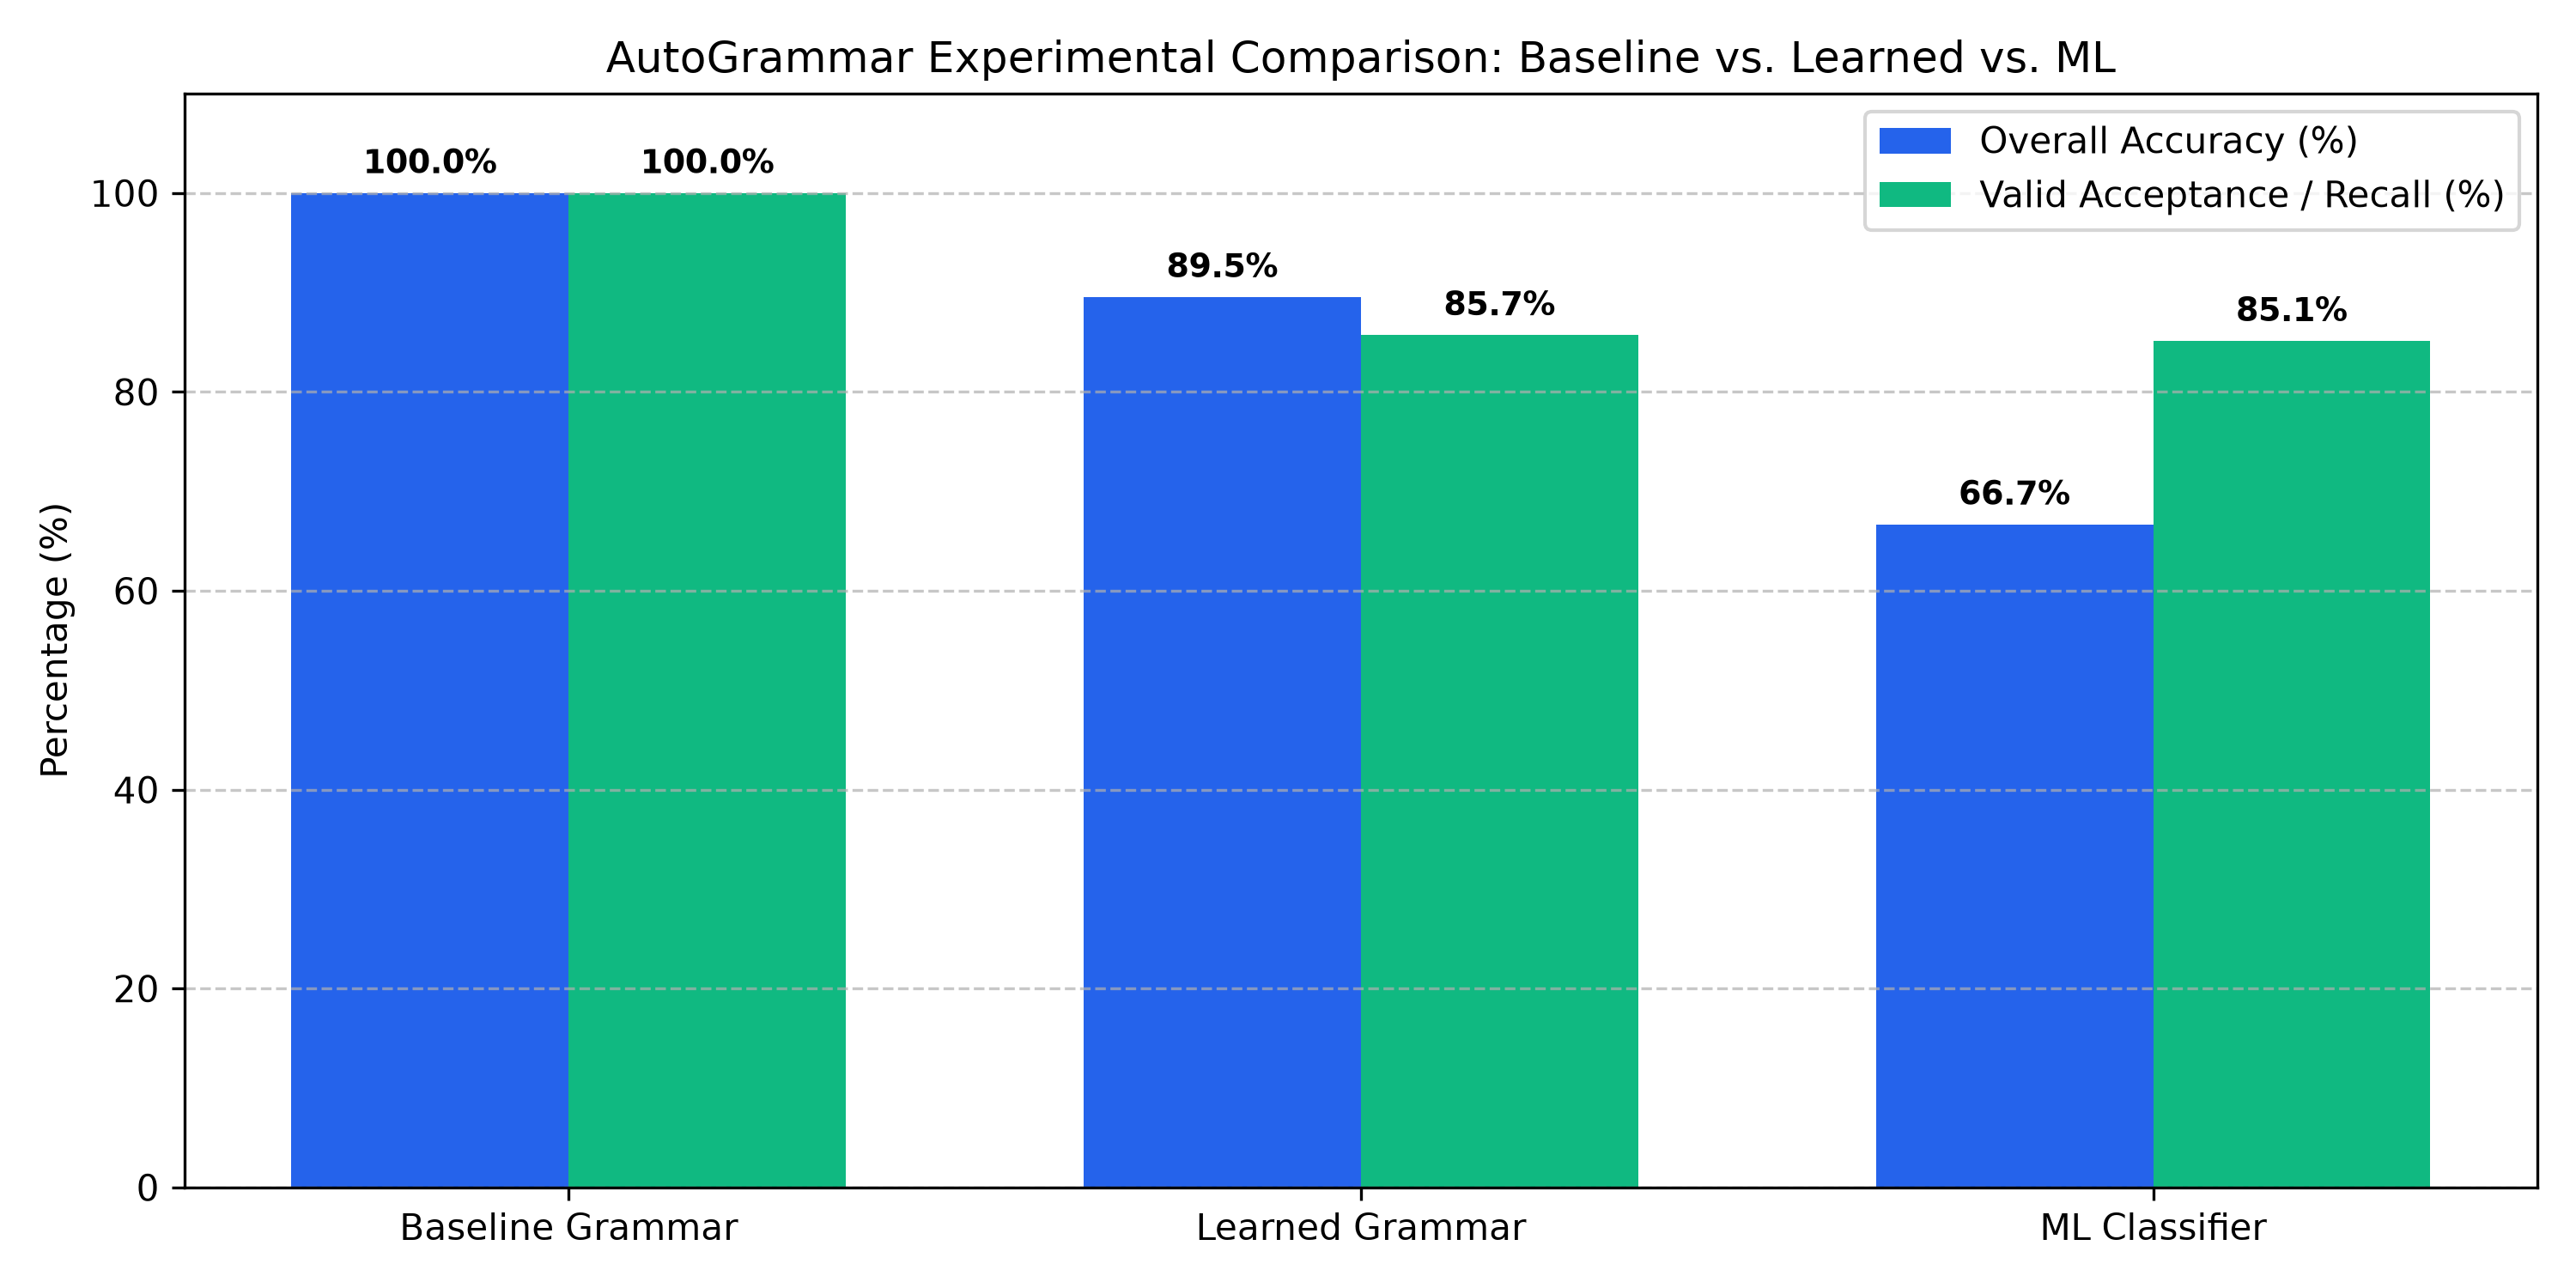
\includegraphics[width=0.75\textwidth]{figures/metrics_comparison.png}
\caption{Comparative performance metrics across Baseline Grammar, Learned Grammar, and ML Classifier.}
\label{fig:metrics}
\end{figure}

\section{Conclusion and Future Work}
AutoGrammar demonstrates that machine learning-based grammar induction can be integrated into compiler pipelines to produce formal, verifiable, and executable domain-specific language parsers. By enforcing template-level disjoint partitioning, we showed that formal rule induction substantially outperforms statistical token classifiers in accuracy, specificity, and explainability.

Future work includes extending the induction engine to probabilistic context-free grammars (PCFGs), incorporating neural semantic proposal models, and supporting cross-dialect SQL adaptations.

\bibliographystyle{plain}
\bibliography{references}

\end{document}
